                       \documentclass[prb,twocolumn,amsmath,longbibliography,amssymb,superscriptaddress]{revtex4-1}

\usepackage[pdftex]{graphics}
\usepackage{graphicx}
\graphicspath{{figures/}}
\usepackage{hyperref}
\usepackage{xcolor}
\usepackage{physics}
\usepackage{subfig}
\usepackage{bm}
\usepackage{caption}

\newcommand{\carlos}[1]{{\color{red} #1}}
\newcommand{\maria}[1]{{\color{blue} #1}}

	
\begin{document}
		
\title{Something fancy...}
\author{Carlos Ortega Taberner}
\affiliation{Department of Physics, Stockholm University, AlbaNova University Center, SE-106 91 Stockholm, Sweden}
\affiliation{Nordita, KTH Royal Institute of Technology and Stockholm University, SE-106 91 Stockholm, Sweden}

\author{Maria Hermanns}
\affiliation{Department of Physics, Stockholm University, AlbaNova University Center, SE-106 91 Stockholm, Sweden}
\affiliation{Nordita, KTH Royal Institute of Technology and Stockholm University, SE-106 91 Stockholm, Sweden}
\date{\today}
		
\maketitle
	


\section{Introduction}



\section{Model.}

As a starting point we consider the model in the BDI class used in reference \cite{Song2014} because it is the simplest model which supports topological phases with winding numbers $\nu = 0,1,2$. Additionaly, we include two symmetry breaking terms, $\kappa$ and $\kappa'$, to obtain an even richer phase diagram and show that our results are not limited to any topological class. The Hamiltonian is then given by
\begin{align}
H =& \sum_{i\alpha,j\beta} c_{i\alpha}^\dagger H_{ij,\alpha \beta} c_{j\beta} \\
H_{ij} =& (m \sigma_x + \kappa \sigma_z)\delta_{ij}  + \frac{1}{2i}\kappa'\sigma_z (\delta_{i-j,1}-\delta_{i-j,-1})\\
&+ \frac{1}{2} t \left[(\sigma_x + i \sigma_y)\delta_{i,j+1} + (\sigma_x - i \sigma_y) \delta_{i,j-1} \right] \\
&+  \frac{1}{2} t' \left[(\sigma_x + i \sigma_y)\delta_{i,j+2} + (\sigma_x - i \sigma_y) \delta_{i,j-2} \right],
\label{bdi_model}
\end{align}
with the corresponding Bloch Hamiltonian being
\begin{align*}
H(k)=&\mqty( \kappa + \kappa' \sin(k) & t' e^{i2k} + t e^{ik}+m \\t' e^{-i2k} + t e^{-ik}+m & -\kappa-\kappa' \sin(k)  ) \\
=& (t' \cos(2k)+t\cos(k)+m)\sigma_x \\
&+ (-t' \sin(2k)-t\sin(k))\sigma_y + (\kappa+\kappa'\sin(k)) \sigma_z.
\end{align*}
For $\kappa = \kappa' = 0$ this Hamiltonian has the following symmetries
\begin{alignat*}{2}
&T = \mathcal{K} ; \quad &&T H(-k) T^{-1} = H(k) \\
&C = \sigma_z\mathcal{K} ; \quad &&C H(-k) C^{-1} = -H(k) \\
&S = \sigma_z ; \quad &&S H(k)S^{-1} = -H(k) 
\end{alignat*}
and therefore it is in the BDI class, where the system has the phase diagram shown in Fig.\ref{bdi_phase_diagram} for $t=0,1$. We also show cuts with the transitions $\nu = 2 \rightarrow 0$ and $\nu = 1 \rightarrow 2$ for different values of $\kappa,\kappa'$.  For $\kappa' \neq 0$ only $C$ is preserved and the system belongs now to the $D$ class. The $Z$ invariant transforms into a $Z_2$ invariant and the original $\nu = 2,0$ phases become equivalent. For $\kappa \neq 0$ only $T$ is preserved and the system is in the trivial AI class, where all zero-energy modes split.
\begin{figure}[h!]
\centering
\makebox[0pt]{
\subfloat[$t = 1,\kappa =\kappa'=0$]{
  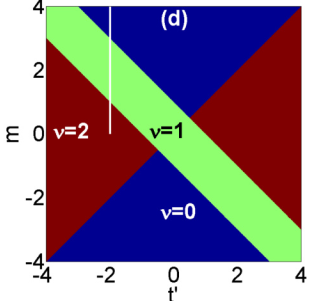
\includegraphics[width=35mm]{bdit1}
}
\subfloat[$t=0,\kappa = \kappa'=0$]{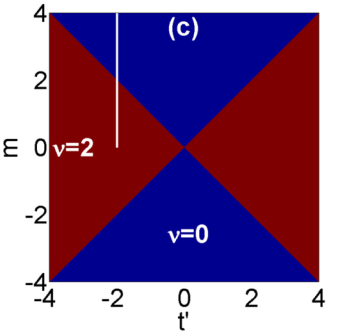
\includegraphics[width=35mm]{bdit0}
}
}\hspace{0mm}

\makebox[0pt]{
\subfloat[$t = 1,t'=1,\kappa =\kappa'=0$]{
  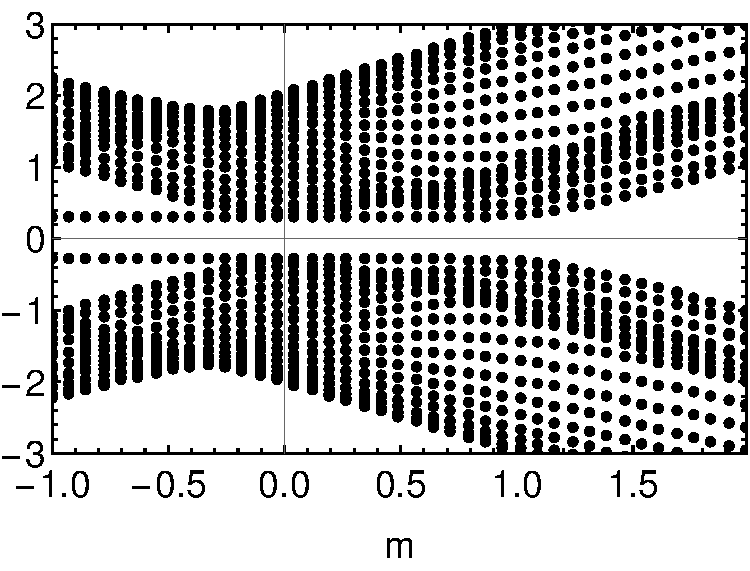
\includegraphics[width=35mm]{1_c.pdf}
}
\subfloat[$t=0,t'=1,\kappa = \kappa'=0$]{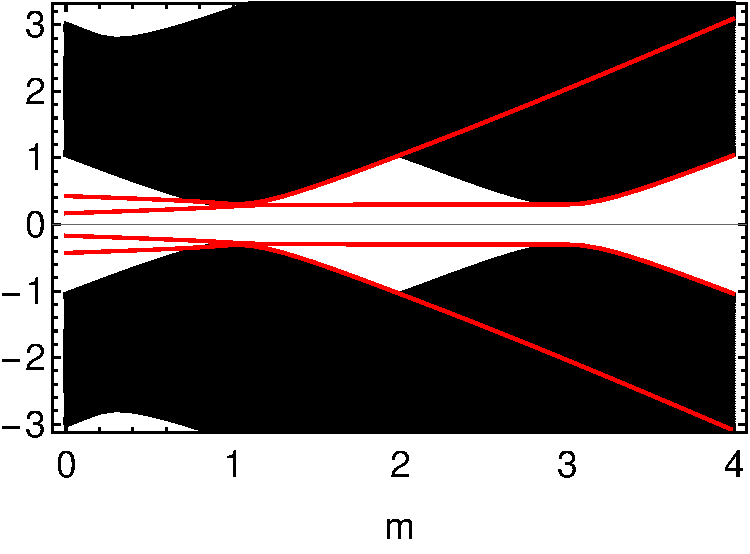
\includegraphics[width=35mm]{1_d.pdf}
}
}\hspace{0mm}

\makebox[0pt]{
\subfloat[$t = 1,t'=1$, $\kappa = 0,\kappa'=0.3$]{
  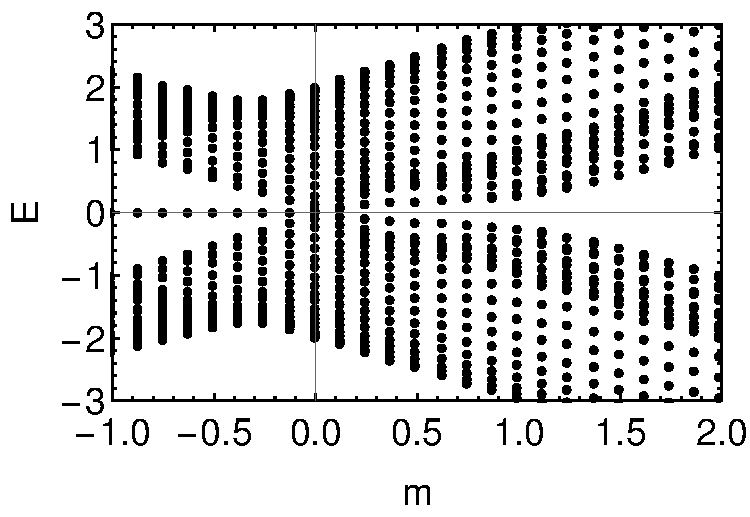
\includegraphics[width=35mm]{1_f.pdf}
}
\subfloat[$t=0,t'=1$, $\kappa = 0.3,\kappa'=0$]{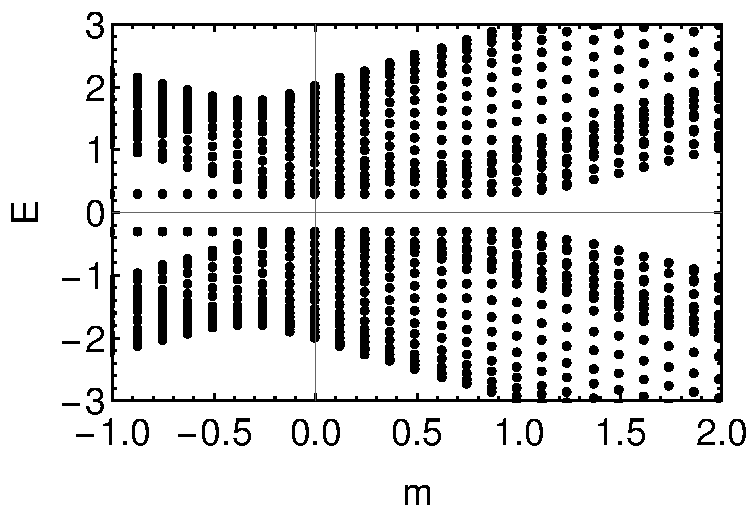
\includegraphics[width=35mm]{1_g.pdf}
}
}
\caption{Phase diagram for the system in the $BDI$ class showing the winding number of each region and surface energy spectrum for two different cuts in the phase diagram for different values of $\kappa,\kappa'$.}
\label{bdi_phase_diagram}
\end{figure}

\section{Geometric phase and Entanglement spectrum}
Consider a quadratic Hamiltonian in one dimension
\begin{equation}
\mathcal{H} = \sum_{ij,\alpha\beta} c_{i\alpha}^\dagger H_{ij,\alpha \beta}c_{j\beta}.
\end{equation}
We can obtain the single-particle eigenstates as
\begin{align*}
\sum_{j\beta}H_{ij,\alpha\beta} u^{p\mu}_{j\beta} = E_{p\mu} u_{i\alpha}^{p\mu},
\end{align*}
where $[U]_{j\beta,p\mu} = u^{p\mu}_{j\beta}$ is the unitary matrix that diagonalizes $H$. The polarization can be obtained as the many-body average of position operator, regularized for periodic boudnary conditions \carlos{resta}
\begin{align*}
\expval{X} = -\frac{L}{2\pi} \rm{ Im\, Ln }\bra{\Psi_0}e^{i \frac{2\pi}{L}\hat{X}}\ket{\Psi_0},
\end{align*}
where $\ket{\Psi_0}$ is the many-body ground state and $\hat{X}$ is the sum of all the single-particle position operators.
Using that the ground state is a Slater determinant of the single-particle eigenstates it can be rewritten as
\begin{align*}
\expval{\hat{X}} = -\frac{L}{2\pi} \rm{Im \, Ln}\, {\rm det} S,
\end{align*}
where 
\begin{equation}
S_{p\mu,q\nu} = \sum_{j\alpha}u^{p\mu\, \ast}_{j \alpha} e^{-i\frac{2\pi}{L}j}u^{q\nu}_{j \alpha}
\end{equation}
and the determinant is taken restricting $S$ to only the occupied eigenstates. The geometric phase can now be obtained as
\begin{equation}
\gamma = \expval{\hat{X}}\frac{2\pi}{L}
\end{equation}

The correlation function in position space is given by
\begin{align*}
C_{ij}^{\alpha \beta} = \expval{c_{i\alpha}^\dagger c_{j\beta}}.
\end{align*}
In terms of the fermions that diagonalize the Hamiltonian, 
\begin{align*}
& \gamma_{i\alpha} = \sum_{j\beta}u_{j\beta}^{i\alpha \, \ast} c_{j\beta} \\
& c_{i\alpha} = \sum_{j\beta} u^{j\beta}_{i\alpha} \gamma_{j\beta}
\end{align*}
we have
\begin{align*}
C_{ij}^{\alpha \beta} =& \sum_{pq,\mu\nu} u^{q\nu }_{j\beta} u^{p\mu \, \ast}_{i\alpha} \expval{\gamma^\dagger_{p\mu} \gamma_{q\nu} } \\
=&  \sum_{p\mu} u^{p\mu }_{j\beta} u^{p\mu \, \ast}_{i\alpha} \expval{\gamma^\dagger_{p\mu} \gamma_{p\mu} } \\
=&  \sum_{p\mu} u^{p\mu }_{j\beta} u^{p\mu \, \ast}_{i\alpha} [1-{\rm sign}(E_{p\mu})]/2.
\end{align*}
The first term is simply a kronecker delta between both sets of indeces. The second term can be rewritten as
\begin{align*}
UD(\abs{D})^{-1}U^\dagger =& UD(D^2)^{-1/2}U^\dagger \\
=& U D U^\dagger (U D^2 U^\dagger)^{-1/2} \\
=& H(H^2)^{-1/2},
\end{align*}
where $D$ is the diagonal Hamiltonian, $H=UDU^\dagger$. Finally the correlation function can be obtained in position space as
\begin{align*}
C_{ij}^{\alpha \beta} =& \frac{1}{2}\left[I - H/ (H^2)^{-1/2} \right]_{ij, \alpha \beta}
\end{align*}

\section{Entanglement spectrum}
\carlos{motivation}

We will obtain the entanglement spectrum by following Peschel's method. Consider a quadratic Hamiltonian in one dimension
\begin{equation}
H = \sum_{ij,\alpha\beta} c_{i\alpha}^\dagger H_{ij,\alpha \beta}c_{j\beta}.
\end{equation}
The correlation function in position space is given by
\begin{align*}
C_{ij}^{\alpha \beta} = \expval{c_{i\alpha}^\dagger c_{j\beta}}
\end{align*}
and the full correlation function is nothing else than the projector onto the occupied bands
\begin{align*}
C_{ij}^{\alpha \beta} =& \frac{1}{2}\left[I - H/ (H^2)^{-1/2} \right]_{ij, \alpha \beta}
\end{align*}
The entanglement spectrum is then obtained as the spectrum of the subsystem correlation function obtained by bisecting the system into two equal parts. 

\carlos{Explain a bit more ES and plots.}

\section{Homogeneous system}

For symmetry-protected topological systems in one dimension there is a well-known relation between the entanglement spectrum  (ES) and the geometric phase. The geometric phase, which is quantized, is zero whenever there is an even number per edge of eigenvalues at $\xi = 1/2$, and $\pi$ when the number is odd. Beyond symmetry protected systems there have been observations of similarities between the midgap eigenvalue of the entanglement spectrum and the geometric phase \cite{Ryu2006,Huang2012,Huang2012-2}, which in the case of the fully dimerized model becomes an exact identity \cite{Ryu2006}. 

The entanglement spectrum eigenstates can be classified as bulk (with eigenvalues $\xi_{b} = 0,1 $) or edge states (with eigenvalues $\xi_{l,r} \neq 0,1$), which are localized in one of the edges. Note that any eigenstate with eigenvalue different from zero or one we refer to as edge state, and not only the ones at $\xi=1/2$. Consider the combination of all eigenvalues localized in one of the edges modulo one,
\begin{equation}
\chi = \sum_{i \in l} \xi_l \quad {\rm mod} \quad 1. 
\end{equation}
As we will show below, for systems where the ES has more than one edge state per edge one can find the geometric phase in the thermodynamic limit as
\begin{equation}
\lim_{L \rightarrow \infty}\gamma/2\pi =\lim_{L \rightarrow \infty} \chi
\label{mainl}
\end{equation}
In the examples studied in references \cite{Ryu2006,Huang2012,Huang2012-2} most of the edge states sit close to the bulk bands and therefore give a small contribution, which explains why the relation between the midgap eigenvalue and the geometric phase was almost an identity and why it breaks as we go deep into the trivial state. Alternatively, using that the entanglement spectrum is particle-hole symmetric for homogeneous systems we can express $\chi$ as
\begin{equation*}
\chi = \frac{1}{2} \left( \sum_{i\in l}\xi_i-\sum_{i\in r}\xi_i \pm \sum_{i\in b}\xi_i  + N \right) \quad {\rm mod} \quad 1,
\end{equation*}
where $N$ is the total number of electrons in the ground state and the sign on the bulk term is irrelevant since $-1/2 \, {\rm mod} \, 1 = 1/2 \, {\rm mod} \, 1$. This form is preferable when doing numerics because it is difficult to differentiate between edge modes and bulk modes since the latter can acquire a finite eigenvalue due to finite size effects or numerical errors. In Fig.\ref{bdi20} we show for several cases how Eq. \ref{mainl} holds up to finite size errors. The ES does not have therefore enough information to build up the geometric phase, but one needs to look at the localization structure of the edge states. One drastic example of this can be seen in figures \ref{bdi20}.b and \ref{bdi20}.c , where two ES that are almost identical result in a very different geometric phase. 

\begin{figure}[h!]
\centering
\makebox[0pt]{
\subfloat[$t = 0, t' = 2, \kappa = 10^{-5}$]{
  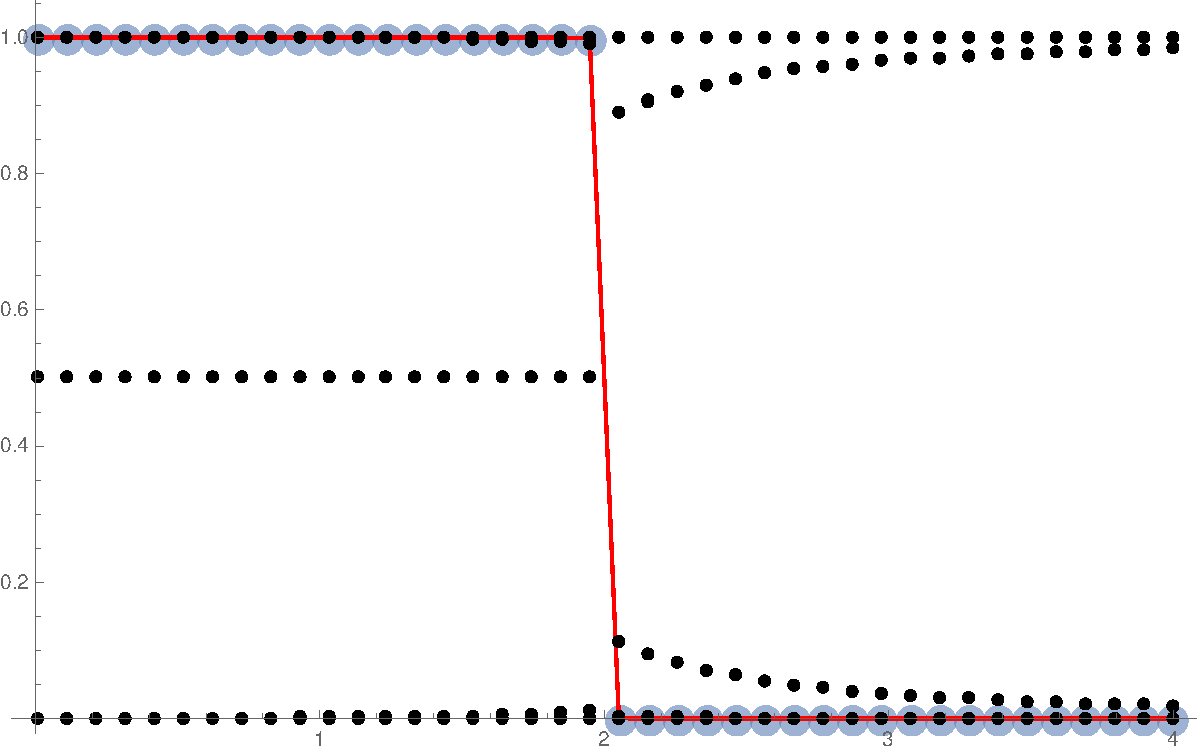
\includegraphics[width=35mm]{bdi20.pdf}
}
\subfloat[$t = 0, t' = 2, \kappa = 0.3$]{
  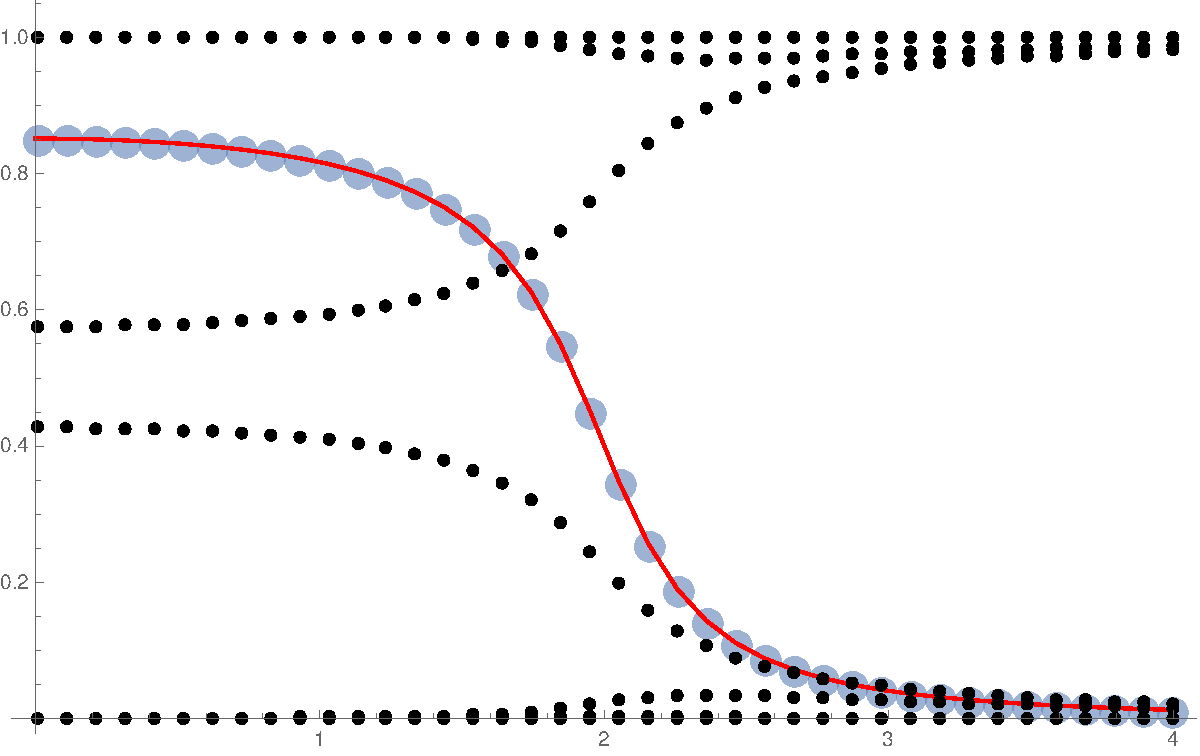
\includegraphics[width=35mm]{ai20.pdf}
}
}\hspace{0mm}

\makebox[0pt]{
\subfloat[$t = 0, t' = 2, \kappa = 0.3$]{
  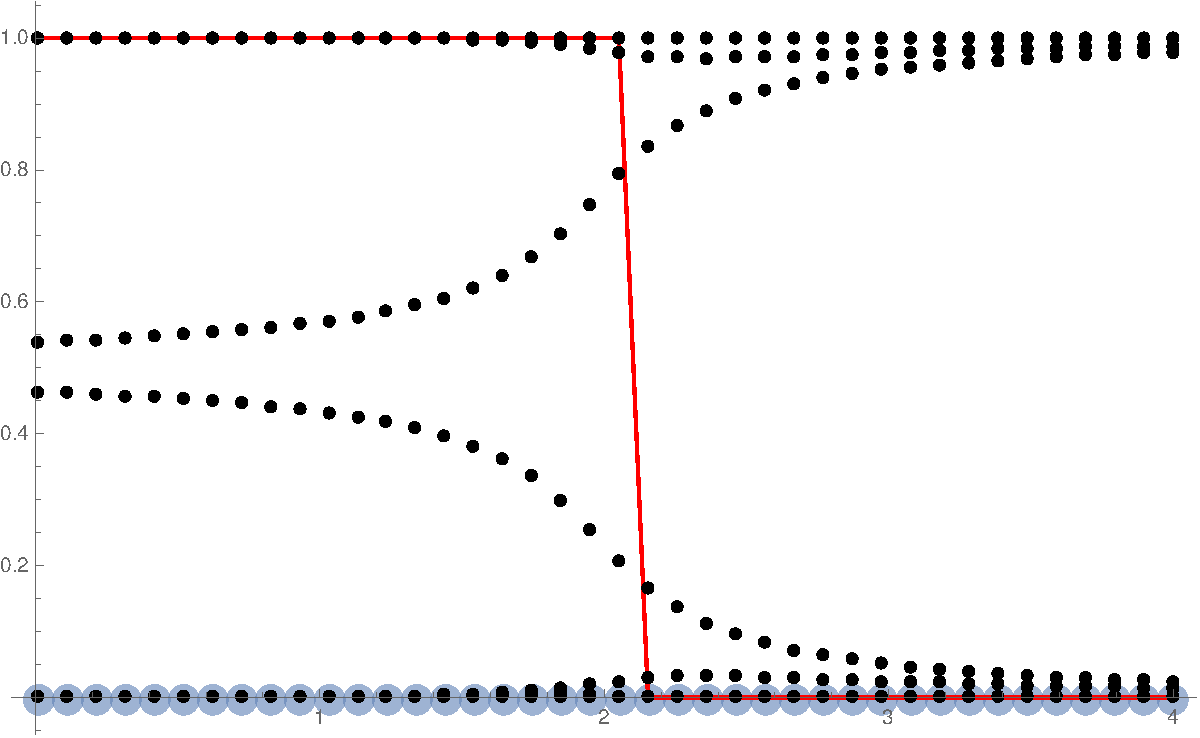
\includegraphics[width=35mm]{d20.pdf}
}
}
\caption{Entanglement spectrum (black), Berry phase (red) and $\chi$ (blue) for different cuts of the $H_{BDI}$. a) with $\kappa = 0,\kappa'=0$ in the $AIII$ class, b) with $\kappa'=0$ in the $AI$ class and c) with $\kappa = 0$ in the $D$ class. }
\label{bdi20}
\end{figure}

This relation between the geometric phase and the entanglement spectrum is a consequence of an identity between the geometric phase and the many-body entanglement spectrum found for infinite chains \cite{Zaletel2014}. In Appendix A we modified this derivation to account for the periodic boundary conditions we use and show how their result reduces to Eq. \ref{mainl} when expressing it in terms of the ES.


\begin{figure}[h]
\centering
\makebox[0pt]{
\subfloat[$t = 0, t' = 2, \kappa = 0.3$]{
  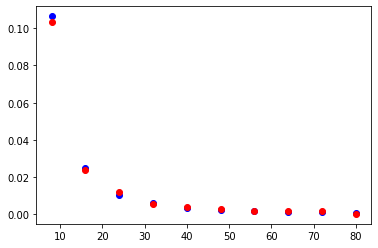
\includegraphics[width=65mm]{scaling_cut_disavg.png}
}
}
\caption{}
\label{disorder}
\end{figure}

\section{Inhomogeneous systems}

In reference \cite{Zaletel2014} translational invariance was used to derive Eq. \ref{zaletel} in Appendix A, and as a result Eq.\ref{mainl} is no longer correct when it is broken. This can be argued in the following way. Weak disorder will modify the entanglement spectrum but not the charge assignment. Without translational invariance the entanglement spectrum will depend on where is the cut placed on the ring, even though the ground state, and therefore the geometric phase, will not. Therefore there cannot be an equivalence between them. Instead, we found that one can still obtain the geometric phase by considering the average over all spatial cuts of expression \ref{mainl}.

In order to test this we take the model we used in the previous section and we promote every parameter to a position-dependent quantity, by adding a random part. In Fig.\ref{disorder} we show $\gamma-\expval{\chi}_{\rm cuts}$ for increasing system size. Note that we do the calculation for a particular disorder configuration for each size. We found that $\expval{\chi}_{\rm cuts}$ converges much faster than the geometric phase and that the difference scales as $O(L^{-2})$, which is the same scaling we find in the homogeneous system. We compared this result with a disorder average $\gamma - \expval{\chi}_{\rm{disorder}}$ and found that, even though we are comparing different disorder configurations, the disorder average and the cut average give the same error, which implies that it must come exclusively from finite size effects in computing the geometric phase, since is the only thing in common. One could think that this cut average is some sort of disorder average, but that is however not correct. In Fig.\ref{cuts} we show the case with a continuous position-dependent potential, plotted in Fig.\ref{cuts}.a, on top of the homogeneous model. In Fig.\ref{cuts}.b we show $\chi_i$ for two cuts where the left edge is either in the positive or negative potential region. As we can see in Fig.\ref{cuts}.c for any intermidiate cut, $\chi_i$ goes continuously from one value to the other. Here we encounter a new problem, since $\chi_i$ only makes physical sense as an angle, there are two paths between the two points. Below the phase transition we find that $\chi_i$ oscillates around $1/2$ while above the phase transition it does so around $0$. By redifining the range of values so that they do not cross $0$ and then averaging we obtain the same result as for the disordered system, that $\gamma-\expval{\chi}_{\rm cuts} \sim O(L^{-2})$. This is only well defined in the continuous limit and can potentially pose problems for finite systems and discontinuous terms, like with disorder. However, as long as the deviations are small and we have $|\expval{\gamma-\chi}|<1/2$, which has been the case so far, one only has to consider two averages, the one with $\chi_i \in [0,1)$ and the one with $\chi_i \in [-1/2,1/2)$, although at the moment there is no indication of which of the two numbers will result on the geometric phase.


\begin{figure}[h!]
\centering
\makebox[0pt]{
\subfloat[]{
  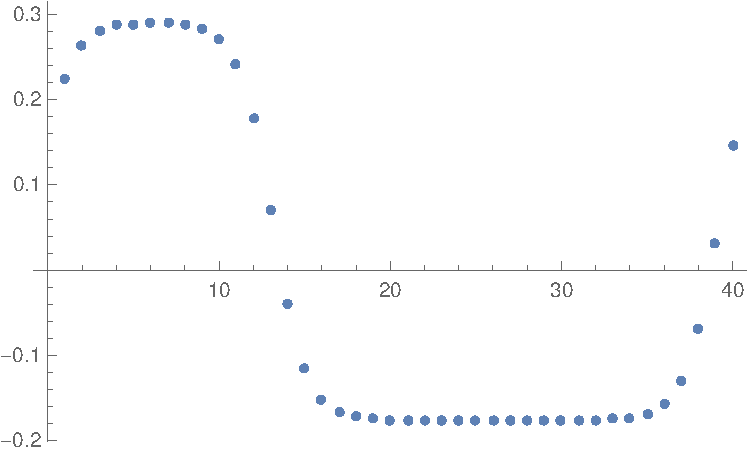
\includegraphics[width=40mm]{profile.pdf}
}
}\hspace{0mm}

\makebox[0pt]{
\subfloat[]{
  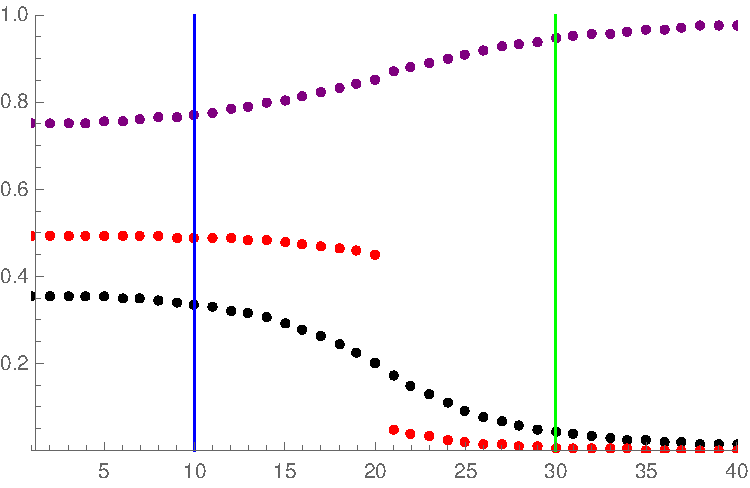
\includegraphics[width=40mm]{extreme_es.pdf}
}
\subfloat[]{
  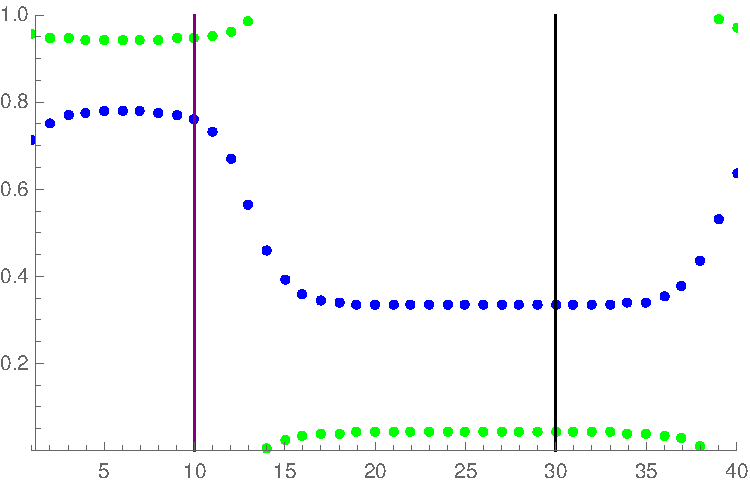
\includegraphics[width=40mm]{cut_es.pdf}
}
}


\caption{a)Profile used for $\kappa_i$ . b)$\chi_i$ for two cases where we place the left cut deep in either the region with positive or negative $\kappa_i$, and geometric phase in red, showing a phase transition. c)$\chi_i$ for all different possible cuts using the parameters $m=1$ (blue) and $m=3$ (green)}
\label{cuts}
\end{figure}

The results in Fig.\ref{disorder} are obtained for weak disorder, where the ES is not modified much. For stronger disorder or other types or inhomogeneous perturbations that strongly modify the ES we run into the issue that $\chi$ is defined modulo $1$ and therefore the cut average is not well-defined. The cut average depends on the range considered for the values of $\chi$. We observed that $\chi$ oscillates around the value of the geometric phase. For weak disorder and continuous inhomogeneous perturbations, where one can follow the path of $\xi$ as we run through the different cuts one can use this information to set the numerical range and obtain the correct result for the geometric phase. However for stronger disorder or discontinious perturbations this does not work. The reason $\chi$ is defined modulo $1$ is to get rid of the contribution from the bulk states, as otherwise it is very difficult to numerically classify between bulk and edge state. If we found another way of getting rid of the bulk contribution then $\chi$ and its cut average would be uniquely defined. 
One can explot the fact that, even in the inhomogeneous case, the ES has a type of particle-hole symmetry. If $\xi$ is an eigenvalue for a cut in $s$ then $1-\xi$ is an eigenvalue of the cut in $s+L/2$. This means that all the information is already contained in half of the spectrum. Using the lower half of the spectrum ensures that we have all the information about the edge eigenstates but the bulk contribution vanishes. This is however only valid when there is a gap between the two halfs of the spectrum at any cut $s$.

Alternative one can set a threshold for the eigenvalues we consider in order to avoid the bulk contribution, which will be a good approximation as long as the ES does not have eigenvalues close to the bulk bands, typically close to the trivial phase, and phase transitions. 

\section{Superconducting systems}

The proof in Ref.\cite{Zaletel2014} also breaks down for superconducting systems. However, as we did for systems without translational invariance, one can extend expression \ref{mainl} for systems with pairing terms as well. Since one computes the geometric phase from the single-particle Bogoliubov-de Gennes Hamiltonian, we can obtain the correspondent entanglement spectrum and use expression \ref{mainl} to obtain the geometric phase. Take for example the kitaev chain, with the following Hamiltonian
\begin{align*}
H =& -\mu \sum_{i} c_i^\dagger c_i - t \sum_{i}\left( c_{i+1}^\dagger c_i + {\rm h.c.}\right) \\
&+  \sum_{i}\left( \Delta c_{i} c_{i+1} + {\rm h.c.}\right).
\end{align*}
Using the spinor $\phi_i^\dagger = (c_i^\dagger, c_i)$, we can rewrite the Hamiltonian as
\begin{align*}
&H = \frac{1}{2}\sum_i \phi^\dagger_i H_{BdG,ij} \phi_j,\\
&H_{BdG,ij} = -\mu \tau_z \delta_{ij} - (t \tau_z + i\Delta \tau_y )\delta_{i,j+1}- (t \tau_z - i\Delta \tau_y)\delta_{i,j-1}.
\end{align*}
Note that by taking $t' = \kappa = \kappa = 0$ in the BDI model, Eq. \ref{bdi_model}, we obtain
\begin{align*}
H_{ij} =& m \sigma_x\delta_{ij} + \frac{1}{2} t \left[(\sigma_x + i \sigma_y)\delta_{i,j+1} + (\sigma_x - i \sigma_y) \delta_{i,j-1} \right],
\end{align*}
which is just the Bogoliubov-de Gennes Hamiltonian of the Kitaev chain by rotating $x$ into $z$ and identifying $\mu = -m, t_{\rm Kit} = -t_{BDI}/2, \Delta = -t_{BDI}/2 $. From Fig.\ref{bdi_phase_diagram} we see that the $BDI$ model transitions from $\nu = 1$ to the trivial phase at $t=0, m=\pm t_{BDI}$, or alternatively, when $\mu = \pm 2 t_{Kit}$, which is the known result for the Kitaev chain. Therefore the results already shown for the BDI model studied here are also applicable to the Kitaev chain.  

\bibliography{references}	
	
\appendix

\section{Appendix A}
	
Consider a chain with periodic boundary conditions. A Schmidt decomposition for two bipartite cuts gives the ground state
\begin{equation}
\ket{\psi} = \sum_{p,q} \ket{p,q}_A s_p \ket{p,q}_B s_q,
\end{equation}
where we assume that the size of each subsystem is big enough so that the cuts can be considered independent of each other. We can now take subsystem B and glue its ends together to obtain the ground state of a ring with a single cut. If we include a flux threading inside the ring we obtain
\begin{equation}
\ket{\psi^\phi} = \sum_p s_p \ket{p,p}_B e^{i\phi Q_p},
\end{equation}
The many-body states $\ket{p,p}_B$ can be built by occupying the different ES eigenstates and are therefore characterized by a set of occupying numbers $\{n\}_p$. The many-body entanglement spectrum can also be expressed in terms of the single-particle one \cite{Alexandrinata2011} as
\begin{align}
s_p^2 =& \prod_{i \in {\rm occ}} \xi_i \prod_{i \in {\rm empty}}(1-\xi_i) \\
=& \prod_i (1-\xi_i)\left(\frac{\xi_i}{1-\xi_i} \right)^{n_i}
\end{align}
And the charge can be assigned so that $Q_p = \sum_{\alpha = b,l,r} q_\alpha\sum_{i \in \alpha} n_i$ with the constrain that $q_r,\pm q_b = q_l-1$ \textcolor{red}{Why?}. As the main result of \cite{Zaletel2014} the geometric phase is then found to be
\begin{align}
e^{i\gamma} = e^{2\pi i \sum_p s_p^2 Q_p}  \bra{\psi^0}\ket{\psi^{2\pi}},
\label{zaletel}
\end{align}
where the monodromy is given by
\begin{align}
\bra{\psi^0}\ket{\psi^{2\pi}} =& \sum_p s_p^2 e^{2\pi i Q_p}.
\end{align}
Consider the exponential term
\begin{align*}
e^{2\pi i (q_L N^p_l + (1-q_l)(N^p_r+N^p_b))} =& e^{2\pi i (q_l N^p_l + (1-q_l)(N-N^p_l))} \\
=& e^{4\pi i q_l N^p_l}e^{2 \pi i (N-N^p_l)}e^{-2\pi i q_l N },
\end{align*}
where $N^p_\alpha = \sum_{i \in \alpha} n_i$ and the total number of electrons, $N = \sum_{\alpha = b,l,r} N^p_\alpha$, is independent of $p$. We will consider two natural choices, $q_l = 1,1/2$, for which we have
\begin{align}
\bra{\psi^0}\ket{\psi^{2\pi}} =& 
\begin{cases}
1 & \text{for} \quad q_l = 1 \\
e^{N\pi i} & \text{for} \quad q_l = 1/2,
\end{cases}
\end{align}
where we used that $\sum_p s_p^2 = 1$. The change in the monodromy between both choices is accompanied by a change in the exponential term in Eq.\ref{zaletel}, so that both charge choices are equivalent.

Expressing the contribution of the many-body entanglement spectrum to the geometric phase in terms of the ES, we have
\begin{align*}
\gamma' = 2\pi \sum_{n_i = 0,1} \left(\sum_{i } n_i q_i\right) \left(\prod_m (1- \xi_m)\left(\frac{\xi_m}{1-\xi_m} \right)^{n_m} \right) ,
\end{align*} 
Consider now its derivative with respect to a particular entanglement eigenvalue
\begin{align}
\frac{1}{2\pi}\frac{\partial \gamma'}{\partial \xi_p} =& \sum_{\{n_k\}=0,1}\left(\sum_{i } n_i q_i\right)\frac{n_p - \xi_p}{\xi_p^{1-n_p}(1-\xi_p)^{n_p}}\\
&\times \left(\prod_{m\neq p} (1- \xi_m)\left(\frac{\xi_m}{1-\xi_m} \right)^{n_m} \right)
\end{align}
where
\begin{equation}
 \frac{n_p - \xi_p}{\xi_p^{1-n_p}(1-\xi_p)^{n_p}} = 
  \begin{cases}
    -1, & \text{for } n_p=0 \\
    1, & \text{for } n_p = 1 \\
  \end{cases}	
\end{equation}
Therefore we have
\begin{align*}
\frac{1}{2\pi}\frac{\partial \gamma'}{\partial \xi_p} =& -\sum_{\substack{\{n_{k\neq p}\}=0,1 \\ n_p = 0}}\left(\sum_{i \neq p} n_i q_i\right)\prod_{m\neq p} (1-\xi_m)\left( \frac{\xi_m}{1-\xi_m} \right)^{n_m} \\
&+ \sum_{\substack{\{n_{k\neq p}\}=0,1 \\ n_p = 1}}\left(\sum_{i \neq p} n_i q_i +q_p\right) \prod_{m\neq p} (1-\xi_m)\left( \frac{\xi_m}{1-\xi_m} \right)^{n_m} \\
=&q_p\sum_{\{n_{k\neq p}\}=0,1} \prod_{k\neq p} (1-\xi_k)\left( \frac{\xi_k}{1-\xi_k} \right)^{n_k} \\
\end{align*}
Expand now the sum  for another occupation number $n_{p'} = 0,1$ 
\begin{align*}
\frac{1}{2\pi}\frac{\partial \gamma'}{\partial \xi_p} =& q_p\sum_{\substack{n_{k \neq p \neq p'}=0,1\\ n_{p'}= 0}} (1-\xi_{p'})\prod_{k\neq p,p'} (1-\xi_k)\left( \frac{\xi_k}{1-\xi_k} \right)^{n_k} \\
&+ q_p\sum_{\substack{n_{k \neq p \neq p'}=0,1\\ n_{p'}= 1}} \xi_{p'}\prod_{k\neq p,p'} (1-\xi_k)\left( \frac{\xi_k}{1-\xi_k} \right)^{n_k} \\
 &=q_p\sum_{\substack{n_{k \neq p \neq p'}=0,1}} \prod_{k\neq p,p'} (1-\xi_k)\left( \frac{\xi_k}{1-\xi_k} \right)^{n_k} 
\end{align*}
doing this for the rest of the occupation numbers we obtain 
\begin{equation}
\frac{1}{2\pi}\frac{\partial \gamma'}{\partial \xi_p} = q_p,
\end{equation}
so that 
\begin{align*}
\gamma =& \gamma' - i\log(\bra{\psi^0}\ket{\psi^{2\pi}})\\
=& \sum_{i}q_i \xi_i - i\log(\bra{\psi^0}\ket{\psi^{2\pi}})\\
\end{align*}
and we have recovered equation \ref{mainl}. 

\end{document}
